\chapter{Analyzing the CIDR Report} % BETTER TITLE
\label{chap:method}

This chapter describes the methods employed to analyze the effectiveness of the
CIDR Report. The chapter begins with a high-level overview of the analytical
approach to impart a conceptual understanding of this thesis' analytical
methods to the reader. Following this, the sources of data used to perform the
analysis and the process used the gather the data are described. Steps taken to
preprocess the collected data to bring it into a normalized, canonical form for
analysis are explained. Following this, the implementation of the CIDR Report's
aggregation report is explained. Finally, the process used to analyze the data
gathered from the CIDR Report and from reimplementing the aggregation report is
explained. This is the process that is used to generate the data and analyses
that are described and explored in the following chapter.

\section{Analytical Approach}

% be sure to avoid value-laden terminology within this

The general intuition in analyzing the effectiveness of the CIDR Report is
conveyed by the simple question: \emph{do autonomous systems change their
behavior, as measured by the number of aggregable routes they advertise into
the routing table, after appearing on the CIDR Report?} If the hypothesis that
the CIDR Report was effective in controlling routing table growth based on the
social forces or reputation in the Internet operator community holds, then the
behavior of ASes that appear on the CIDR Report should differ---becoming more
aggregated---compared to the behavior of ASes that never appear on the CIDR
Report. This can be viewed as a quasi-experiment \cite{Babbie:2003uq}, with
ASes that appear on the CIDR Report composing the treatment group and ASes that
never appear as the control group. This cannot be viewed as a true natural
experiment or controlled experiment because the ASes in the treatment group are
not randomly selected. The behavior that leads to appearance on the CIDR Report
is typical of large ISPs and so they are disproportionally represented on the
CIDR Report. This non-random appearance of ASes in the treatment group raise
potential validity concerns, and the implications of this are discussed later.

The analysis of the performance of the treatment group could be implemented
very simply by comparing the behavior of a given AS over time, starting when it
first appears on the top thirty aggregation report. The CIDR Report emails
transmitted to mailing lists weekly contain much of the information necessary
to conduct this analysis. Accordingly, I first gathered and coded the data
contained in these emails from network operator mailing list archives. This
information determines which ASes are in the treatment group and when they
appeared.

The CIDR Report emails have two shortcomings that demand the gathering of
additional data about the routing table. The aggregation report contains no
information about ASes that do not appear within the top thirty, requiring
other information to be gathered in order to form a control group. Also, rank
(and thus appearance) is determined by relative ranking rather than absolute
number of routes, and so an AS in the treatment group may leave the top 30
without aggregating simply because other ASes deaggregate more. In order to
measure behavior in terms of routing table slots consumed by an AS, a
non-truncated version of the CIDR Report is required. No archives of the full
report are available, so I instead gathered historic routing table data and
developed my own implementation of the aggregation report. The information from
this generated aggregation report provides the metrics used for analysis of
ASes in both the control and treatment groups for consistency.

Finally, utilizing the information from both the emailed (authoritative) CIDR
Report and the full aggregation report generated from historic routing table
data, I proceed with analysis, characterizing the overall behavior of ASes in
the treatment and control groups, as well as behavior of ASes in both groups
over time in order to observe whether the CIDR Report may have had an effect on
treated AS' behavior.

\section{Data sources \& data collection} %%%%%%%%%%%%%%%%%%%%%%%%%%%%%%%

\subsection{Authoritative CIDR Reports}

The official CIDR Report has been transmitted weekly on Friday afternoons to
network operator communities including the North American Network Operators
Group (NANOG), starting in September 1997. The NANOG community has kept a
public archive, \cite{NANOG} and \cite{NANOG-new}, of all messages sent to its
mailing list since its inception in 1994, capturing all of the CIDR Report
messages in its archive. This archive is an appropriate source of CIDR Reports
as it contains the messages that were actually received by network operators
(and so used to apply social force under the CIDR Report hypothesis).

The indexes of the archives were downloaded and parsed to obtain a set of
message headers containing the sender name, subject, and date of all messages
sent to the NANOG list. This message list was then filtered to create a coding
candidate set containing only messages with a subject line containing the
string ``CIDR R'' in any mix of upper- and lower-case characters.

The full bodies of the messages in the candidate set were downloaded from the
NANOG archives for coding. The coding process consisted of viewing each message
and classifying it as one of:

\begin{itemize}
    \item{an official CIDR Report that appears to be correct,}
    \item{an official CIDR Report that appears incorrect (duplicates, sent on
    the wrong date, containing obviously invalid data, etc.),}
    \item{an email from the operator community praising, criticizing, or
    discussing behavior in the CIDR Report, or}
    \item{none of the above (not of interest).}
\end{itemize}

Following the coding process, emails coded as official and correct CIDR Reports
were parsed by an automated program to extract rank prefix count information
for every AS appearing on the aggregation report. This information was then
stored in a database for later use by other analysis tools.

%%%%% Move this to background?

One benefit of coding the authoritative CIDR Report emails by hand was that it
enabled observation of changes in the CIDR Report's BGP data vantage point and
implementation over time, as well as the transition of stewardship of the
report. The report as originally conceived and implemented by Tony Bates was
used from the first NANOG CIDR Report on 17 September 1996 until 23 August
2002. Geoff Huston then took responsibility for the report on 30 August 2002,
producing a similarly-formatted report but with a new implementation that was
developed without consulting Bates' source code \cite{Huston:2011ys}. The CIDR
Report's vantage points over time are in the table below. The potential
importance of vantage point selection is discussed further in Chapter
\ref{chap:discussion}.

\savenotes
\begin{table}[h]
    \begin{center}
    \caption{CIDR Report vantage point ASes over time}
    \vspace{1em}
    \begin{tabular}{c | c | c}
        AS number & AS Name & Date effective \\
        \hline
        AS 5413 & Xara.net (at MAE-East) & 17 September 1996 \\
        AS 5413 & GX Networks & 15 June 2001 \\
        AS 6447 & Route Views & 30 August 2002 \\
        AS 4637 & REACH & 11 October 2002 \\
        AS 2.0\footnote{AS 2.0 is not visible in the routing table, but peers
        with AS 4777 and AS 4608 \cite{Huston:2011ys}.} & APNIC R\&D & 20 July
        2007 \\
    \end{tabular}
    \label{table:cr_vantage_points}
    \end{center}
\end{table}
\spewnotes

%%%%% End move

\subsection{Routing Table Data}

The University of Oregon Route Views project \cite{Routeviews} was used as the
source of routing table data for generating a full aggregation report. Route
Views gathers multiple views of the Internet routing table as seen by various
major providers that peer with Route Views, and is a commonly used data source
for operational and academic research. Route Views peers change over time, but
typically include most of the default-free zone (DFZ) providers. The
project has been storing routing table archives since November 1997.

Route Views' data sets export the entire Route Views RIB which contains all
routes received from each provider it peers with. This differs from the Huston
CIDR Report implementation \cite{Huston:2011ys} (and possibly from the original
Bates CIDR Report implementation also), which used the best BGP route available
instead of all routes available.

%The multitude of vantage points included in the Route Views data is arguably
%preferable in that it allows more potential aggregation to be visible to the
%CIDR Report algorithm, as discussed in the background section. It is also
%potentially problematic in that it includes ``leaked'' routes---routes not
%intended to be advertised globally---if they are advertised by even one
%provider. Discussion of the variation in routes observed from peers and the
%consequences of this---the potential importance of vantage point---are
%discussed later.

Route Views RIB snapshots are typically generated every two hours, and so a
script was developed to search the archive indexes for the most appropriate
snapshot to download in accordance with the CIDR Report's weekly Friday release
schedule. The script selects the RIB snapshot created most recently after
midnight each Friday. For the cases where RIB files were not found for a given
Friday, the most recently generated RIB from earlier in the same week was
selected instead. Between November 1997 and November 2001, snapshots in ``Cisco
CLI''-format\footnote{Cisco CLI is a text-based RIB format captured by copying
the output of the \texttt{show ip bgp} command from a Cisco router's
command-line interface.} RIBs were downloaded from
\url{route-views.routeviews.org}. After November 2001, MRT-format\footnote{MRT
is a binary RIB format that essentially encapuslates BGP UPDATE messages in a
well-known format for archiving and later analysis. It is currently an
Internet-Draft being developed by the IETF:
\url{http://tools.ietf.org/html/draft-ietf-grow-mrt-14}.} RIBs were downloaded
from \url{route-views2.routeviews.org}. These RIBs were stored for
preprocessing and ultimately the generation of the full aggregation report.

\section{Data preprocessing}

Several preprocessing steps are required to extract and normalize the data from
the Route Views RIB files in order to prepare the data for use in generating
the aggregation report.

First the information required from each RIB snapshot---namely the advertised
prefix, the IP address of the observing peer, and the AS\_PATH associated with
the route---are extracted from the snapshot files using RIPE's libbgpdump
library \cite{libbgpdump} for MRT-format RIB snapshots and CAIDA's straightenRV
tool \cite{straightenrv} for ``Cisco CLI''-format RIB snapshots. The output of
these programs was a plain text representation of the information extracted
from the RIB in the form of (prefix, peer IP address, AS\_PATH) tuples.

Next, these simplified RIB files were processed to canonicalize the AS\_PATH
associated with each prefix. Since AS\_PATH equality is used by the aggregation
report to determine whether the routing policy of two prefixes is the same, a
canonical representation of the AS\_PATH is essential in order to allow
AS\_PATH comparison. There are four steps in the canonicalization process:

\begin{enumerate}
    \item{\textbf{Removal of non-AS\_SEQUENCE elements in the AS\_PATH.} The
    AS\_PATH in a BGP UPDATE message can consist of four types of path segments
    \cite{rfc5065}: AS\_SEQUENCE, an ordered list of ASes traversed by an
    update message; AS\_SET, an unordered set of ASes traversed by an update
    message; AS\_CONFED\_SEQUENCE, an ordered list of private AS numbers
    traversed by an update message in a BGP confederation; and AS\_CONFED\_SET,
    an unordered set of private AS numbers traversed by an update message in a
    BGP confederation.

    AS\_SETs (denoted as \verb!{4,5}! for a set containing AS 4 and 5) are
    included in a set to allow the loop prevention aspect of the AS\_PATH to
    continue to function while indicating that proxy aggregation was peformed
    by a router along the path of the update message
    \cite{draft-deprecate-as-sets-04}. AS\_SETs in the first segment of the
    AS\_PATH make the origin of a route ambiguous because there is more than
    one AS in the origin position of the AS\_PATH. AS\_SET segments are also
    often incorrectly used and add ambiguity to other parts of the AS\_PATH
    \cite{draft-deprecate-as-sets-04}. To resolve such ambiguity, any AS\_SET
    is reduced to a single AS number if it contains only one AS number repeated
    any number of times, or is removed from the AS\_PATH if it contain multiple
    unique AS numbers. As an example, the AS\_SET \verb!{4,4,4,4}! would be
    reduced to \verb!4!, while the AS\_SET \verb!{4,5}! would be discarded.

    AS\_CONFED\_SEQUENCEs (denoted as \verb![4 5]!) and AS\_CONFED\_SET
    (denoted as \verb!(4,5)!) should only contain private AS numbers, should
    not be visible on the public Internet, and contribute no Internet
    topological information about the route, and so are discarded without
    further consideration.

    As an example of all of the transformations applied during this step, the
    path \\
    \verb!1 1 1 2 3 (65535,65533) {4,4}! would become \verb!1 1 1 2 3 4!.
    }

    \item{\textbf{Removal of private AS numbers.} IANA has allocated private AS
    numbers \cite{rfc1930,rfc5398} for ISP internal use and documentation
    purposes, and these AS numbers sometimes appear in the Internet routing
    table. AS numbers within this range are removed from the AS\_PATH.}

    \item{\textbf{Removal of prepended AS numbers.} As discussed earlier,
    AS\_PATH prepending is sometimes used by network operators to make a route
    appear less attractive to the BGP path selection algorithm. A prepended
    AS\_PATH affects traffic engineering but not routing policy, and so
    prepended AS numbers are removed by collapsing contiguous blocks of the
    same AS number into a single entry in the AS\_PATH.

    For example, the path \verb!1 1 1 2 3 3 4! would be collapsed to
    \verb!1 2 3 4!.}

    \item{\textbf{Removal of simple routing loops.} Minor routing loops
    sometimes occur in the BGP routing table, such as when a route traverses a
    provider that uses multiple AS numbers for different parts of their
    infrastructure. These loops are removed following the algorithm used by
    CAIDA in straightenRV\cite{straightenrv}. If a more complex loop is found
    that cannot be resolved using this algorithm, the entire route is
    discarded.

    For example, the path \verb!1 2 3 2 5!, which may have resulted from AS 2
    and 3 belonging to the same operator, is reduced to \verb!1 2 5!. In
    contrast, a more complex loop such as \verb!1 2 3 2 3 4! cannot be resolved
    using CAIDA's heuristic.}
\end{enumerate}

Finally, because this canonicalization process requires a full traversal of the
input RIB in order to produce the canonical RIB, other data sets can be
opportunistically generated during the canonicalization process. The number of
prefixes observed by each Route Views peer are recorded, for each origin AS and
for the entire routing table, to allow later analysis of variation in the
prefixes seen per peer. This information was a helpful debugging tool and
will also be used for the later discussion of the consequences of vantage
point selection.

\section{Implementing the Aggregation Report}

Determining which prefixes in a RIB are aggregable consists of three major
steps. First, a prefix tree data structure containing all advertised prefixes
is constructed in order to establish which prefixes are adjacent to and covered
by other prefixes. Next, the tree is walked recursively aggregate adjacent
prefixes and to classify prefixes that may be aggregated by a covering prefix,
both only in cases where routing policy is not compromised. Finally, counts of
aggregable and total prefixes are attributed to each origin AS. These counts
are then ranked to generate the aggregation report as seen on the CIDR Report.
Each of these steps is described in more detail below.

To construct the binary prefix tree (perhaps more correctly a binary prefix
trie \cite{Wu:2008fk}) containing a set of prefixes that we wish to aggregate
over, the root of the tree must be determined. If prefixes of any length were
allowed then the tree would need to be rooted at 0.0.0.0/0. However, because
IANA has always allocated IP address blocks as Class A or /8 blocks, we
generate the aggregation report by considering each /8 separately. Taking
advantage of this fact will make the implementation of the classification
algorithm more efficient as the entire routing table need not be stored in
memory. Accordingly, the input RIB is sorted on the first octet of the prefix
and processed by the algorithm one /8 at a time.

For each /8, a prefix tree is constructed with the /8 prefix at the root (for
example, 10.0.0.0/8). Then, each prefix in the RIB, as observed by each peer,
is inserted into the tree. Each node contains a prefix, the corresponding
AS\_PATH for that prefix, and pointers to the two more specific sub-prefixes of
the current prefix if they exist. An small example of a prefix tree is shown in
Figure \ref{fig:ex_prefix_tree}.

\begin{figure}
\begin{center}
    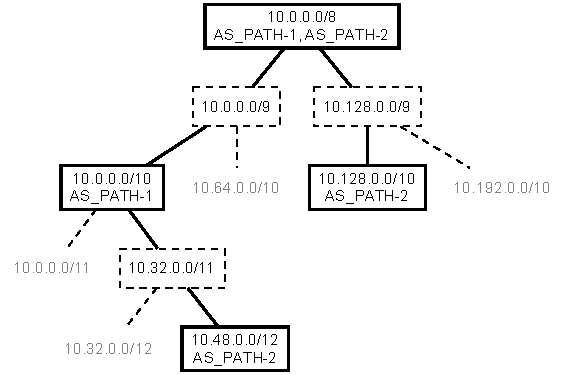
\includegraphics{figures/ex_prefix_tree.pdf}
    \caption[A prefix tree]{A prefix tree for 10.0.0.0/8 and some more specific
    prefixes. Prefixes with solid borders and AS\_PATHs are announced in the
    routing table, and prefixes with dashed borders are placeholders.}
    \label{fig:ex_prefix_tree}
\end{center}
\end{figure}

To insert a prefix into the tree, a cursor is placed at the root and then
advanced to one of the two children of the root, depending on whether the first
bit after the first octet of the IP prefix is a `1' or a `0'. This process is
then repeated recursively at each node the cursor encounters for each
corresponding subsequent bit in the prefix. If at any point a node does not
have a child node that must be traversed to reach the insertion point, a
placeholder prefix is inserted to maintain the tree structure. When the
cursor's depth in the tree is equal to the length of the prefix less the
original eight bits of the /8, the prefix is inserted into the tree. The
insertion process is illustrated in Figure \ref{fig:ex_prefix_tree_insert}.

\begin{figure}
    \subfigure[Bit 9 of the prefix is a `1', so the cursor proceeds to the `1'
    child.]
    {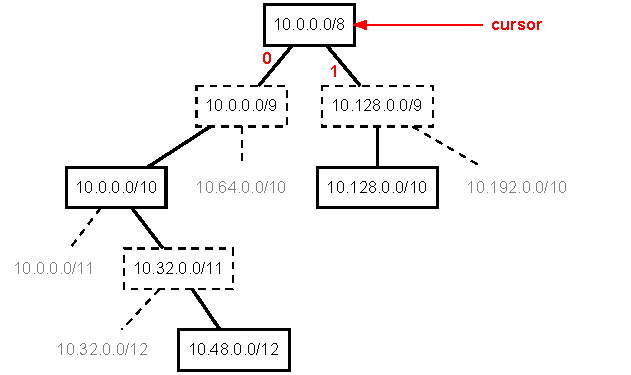
\includegraphics[width=3in]{figures/prefix_insert_gl1.pdf}}
    \subfigure[Bit 10 of the prefix is a `0', so the cursor proceeds to the `0'
    child.]
    {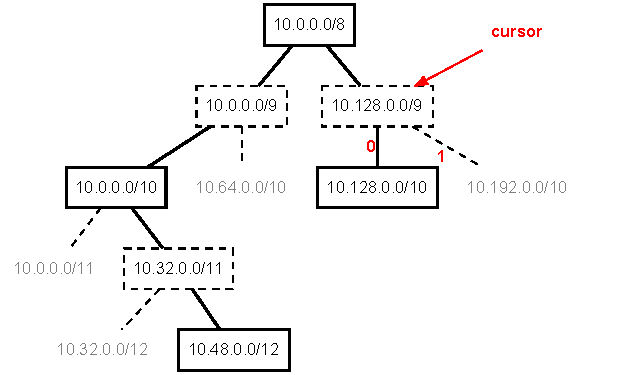
\includegraphics[width=3in]{figures/prefix_insert_gl2.pdf}}
    \subfigure[Bit 11 of the prefix is a `1', so the cursor proceeds to the `1'
    child. The `1' child does not exist, so a placeholder prefix is inserted as
    the `1' child.]
    {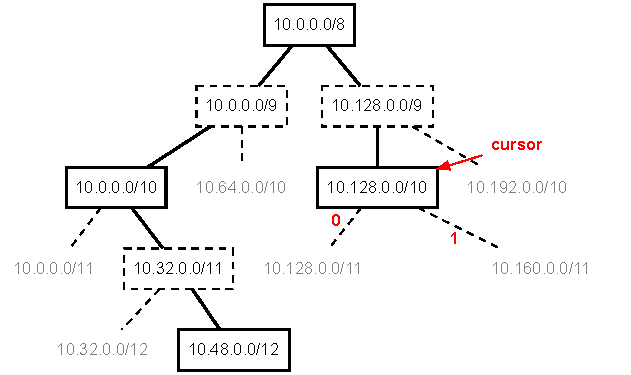
\includegraphics[width=3in]{figures/prefix_insert_gl3.pdf}}
    \subfigure[Bit 12 of the prefix is a `0', so the cursor proceeds to the `0'
    child. The `0' child does not exist. Since the current bit is equal to the
    prefix length (/12) the (non-placeholder) prefix 10.160.0.0/12 is inserted
    as the `0' child.]
    {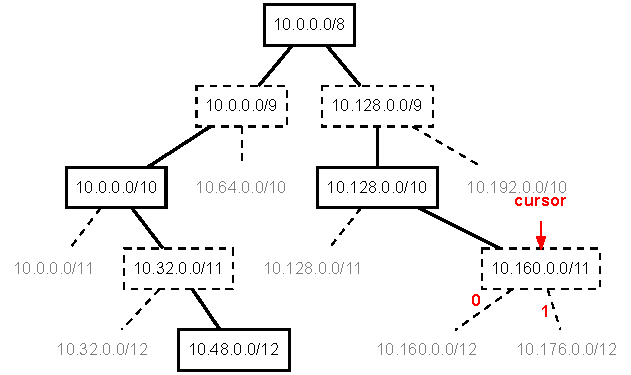
\includegraphics[width=3in]{figures/prefix_insert_gl4.pdf}}
    \subfigure[Insertion of 10.160.0.0/12 is complete.]
    {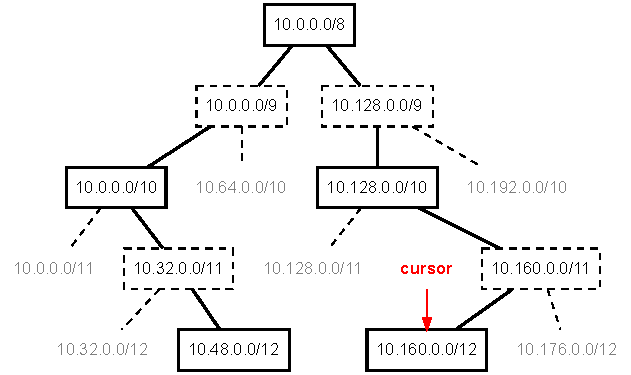
\includegraphics[width=3in]{figures/prefix_insert_gl5.pdf}}
    \caption[Insertion into the prefix tree]{Insertion of 10.160.0.0/12 into
    the prefix tree described in Figure \ref{fig:ex_prefix_tree}. Recall that
    10.160.0.0 is represented as 00001010.10100000.00000000.00000000 in
    binary.}
    \label{fig:ex_prefix_tree_insert}
\end{figure}

Unlike the Huston and likely the Bates implementations of the aggregation
report, this implementation considers all routes available from all peers for a
given prefix in the routing table, instead of just the best route. Thus, for a
given prefix in the tree, there are actually multiple AS\_PATHS stored---one
for each peer that observes the route. This can be viewed logically as several
prefix trees overlaid on top of each other, though the implementation uses
a single tree with multiple AS\_PATHs per prefix. All distinct AS\_PATHs
for a given prefix are gathered from the input RIB and associated with the
prefix before it is installed in the prefix tree.

%This is important in that it allows the most potential aggregation to be
%observed because it does not conflate routes viewed from different peers. For
%example, consider the following topology shown in Figure
%\ref{fig:ex_topology}, and the routes observed from two peers shown in the
%routing table below:
%
%\begin{figure}
%\caption{Example topology and route announcements.}
%\label{fig:ex_topology}
%\end{figure}
%
%% \begin{tabular}{l | l}
%%     prefix        & AS\_PATH \\
%%     \hline
%%     10.0.0.0/8    & 30 20 10 \\
%%     10.0.0.0/9    & 30 20 10 \\
%%     10.128.0.0/9  & 30 20 10 \\
%% \end{tabular}
%%
%% \begin{tabular}{l | l}
%%     prefix        & AS\_PATH \\
%%     \hline
%%     10.0.0.0/8    & 40 10       \\
%%     10.0.0.0/9    & 40 30 20 10 \\
%%     10.128.0.0/9  & 40 30 20 10 \\
%% \end{tabular}
%%
%% \begin{tabular}{l | l}
%%     prefix        & AS\_PATH \\
%%     \hline
%%     10.0.0.0/8    & 40 10    \\
%%     10.0.0.0/9    & 30 20 10 \\
%%     10.128.0.0/9  & 30 20 10 \\
%% \end{tabular}
%
%\begin{figure}
%\caption{Example routing tables based on routes and topology in figure
%\ref{fig:ex_topology}} \label{fig:ex_tables}
%\begin{centering}
%\begin{tabular}{l | l c l | l c l | l}
%    \multicolumn{2}{c}{\textsc{Routes From AS 30:}} & &
%    \multicolumn{2}{c}{\textsc{Routes From AS 40:}} & &
%    \multicolumn{2}{c}{\textsc{Observer's Best Routes:}} \\ prefix        &
%    AS\_PATH & & prefix       & AS\_PATH    & & prefix & AS\_PATH \\
%    \cline{1-2} \cline{4-5} \cline{7-8}
%    10.0.0.0/8    & 30 20 10 & & 10.0.0.0/8   & 40 10       & & 10.0.0.0/8 &
%    40 10 \\ 10.0.0.0/9    & 30 20 10 & & 10.0.0.0/9   & 40 30 20 10 & &
%    10.0.0.0/9 & 30 20 10 \\
%    10.128.0.0/9  & 30 20 10 & & 10.128.0.0/9 & 40 30 20 10 & & 10.128.0.0/9 &
%    30 20 10 \\
%\end{tabular}
%\end{centering}
%\end{figure}
%
%By looking at only the BGP-selected best routes from the observation vantage
%point (the right-most table in Figure \ref{fig:ex_tables}), it's possible to
%conclude that routes aren't aggregable.

Once all of the prefixes in the RIB for the current /8 are inserted into the
prefix tree, the prefix tree is walked recursively to aggregate and classify
aggregable prefixes within the tree. As noted in the background, a prefix is
considered aggregable if it has the same routing policy as a less-specific
covering prefix. The aggregation and classification algorithm was implemented
based on the description of the CIDR Report included in the Report's preamble,
as well as detailed records of the report's operation
\cite{cidr-report-details}. Like the authoritative CIDR Report, routing policy
equality in this implementation of the aggregation report is determined by
comparing AS\_PATH equality.

The general algorithm behind the aggregation and classification process is as
follows. The prefix tree is traversed using post-order recursion and the
following operations are performed on each node before the function returns to
its calling parent (the post-order traversal ensures that children are
aggregated before their parents):

\begin{enumerate}
    \item{Attempt to aggregate children: If the current prefix is a placeholder
    and has two more-specific (child) prefixes announced in the routing table,
    check to see if their AS\_PATHs match. If they do, convert the current
    prefix into a ``true'' (non-placeholder) prefix and mark the children
    prefixes as aggregable.}
    \item{Attempt to aggregate by a covering prefix: Compare the AS\_PATH of
    the current prefix with the AS\_PATH of its nearest less-specific
    (ancestor) prefix . If they match, mark the current prefix as aggregable.}
\end{enumerate}

This process is again logically conducted as though there are multiple separate
but overlaid trees for each Route Views peer/observer AS. The process is
actually implemented by processing all vantage points available at a given
prefix and aggregating and classifying them against other ancestor and child
prefixes visible from the same peer AS. Classifications of aggregability are
made on a per-peer basis, and then must be generalized for the entire prefix.
There is no single way to make this generalization and so a design decision
must be made.

There are two obvious choices for how generalize across each vantage point's
aggregation classification for a given prefix: consider the prefix aggregable
if \emph{any} vantage point considers it aggregable, or only if \emph{all}
vantage points consider it aggregable. The latter option requires consensus
that a prefix be aggregable across all views, while the former allows any claim
of aggregability to stand. Our implementation of the aggregation report
classifies a prefix as aggregable if it is classified as aggregable from
\emph{any} vantage point. While perhaps ``pessimistic'', this approach will
detect and report the maximum amount of aggregation potentially possible.

%\fbox{include note on multihoming/traffic engineering, and whether this
%applies as compared to other efforts., i.e. citadinni}

Finally, when a prefix is marked as aggregable, it must be attributed to the
network that announced the prefix as this network is responsible for the
redundant route announcement. This is normally performed by attributing the
aggregable route to the origin AS---the first AS in the route's AS\_PATH---that
is presumed to be the announcing network. An ambiguous situation arises in the
case of prefixes announced by multiple ASes, a condition known as a multiple
origin AS (MOAS) \cite{Zhao:2001ly}. Again, a design decision must be made for
how to attribute aggregable MOAS prefixes: the MOAS prefixes could be ignored,
the route's behavior could be attributed to one of the origin ASes, or it could
be attributed to all origin ASes. This implementation attributes an aggregable
prefix to each unique AS that announces the prefix.

To attribute deaggregation behavior to each AS, the aggregation report
processor maintains five quantities for each origin AS:

\begin{itemize}
    \item{Announced routes (\emph{announced} or \emph{netsnow}): routes that
    were originally announced in the input RIB. This is the ``netsnow''
    quantity in the aggregation report}
    \item{Withdrawn routes (\emph{widthdrawn}): routes that were covered by
    less specific routes and thus would be withdrawn from the
    ideally-aggregated routing table.}
    \item{Aggregated routes (\emph{aggregated}): routes that did not exist in
    the original routing table, but were synthesized by combining two adjacent
    prefixes into a covering prefix.}
    \item{Total reduction in routes under perfect aggregation (\emph{netgain}):
    computed as $\textit{netgain} = \textit{withdrawn} - \textit{aggregated}$}
    \item{Total advertised routes under perfect aggregation (\emph{netsaggr}):
    computed as $\textit{netsaggr}=\textit{announced} + \textit{aggregated} -
    \textit{withdrawn}$}
\end{itemize}

If a prefix in the prefix tree is marked as aggregable and is originally from
the input RIB, then this prefix is counted as a \emph{withdrawn} route. If a
prefix is synthetic aggregate (not from the input RIB) and not marked as
aggregable, then it is counted as an \emph{aggregated} route.

After all of the RIB's routes are processed, the counts of aggregable routes
attributed to their origin ASes---in the form of a list of tuples containing
the origin AS and the five quantities described above (origin AS, netsnow,
netgain, netsaggr, aggregated, withdrawn)---must be sorted to determine the
ranking of networks as found on the authoritative CIDR Report. The ranking of
ASes on the aggregation report is generated by a primary sort on the netgain
value, the number of aggregable prefixes announced by the AS. The AS with the
greatest netgain value will be hold rank 1 on the aggregation report. To
provide an ordering when networks have the same netgain value, a secondary sort
is performed to rank networks with a lesser netsnow value above networks with a
greater netsnow value if both have the same netgain---these networks are more
deaggregated as a fraction of their total routes. Finally, a tertiary sort is
performed on the AS number as a sort of last resort to produce a canonical
ordering similar to that found on the full, authoritative CIDR Report
\cite{cidr-report-full}. With this final sorting, the aggregation report data
is ready for analysis.

\section{Analyzing the Aggregation Report}
\label{sec:method_agg_report_analysis}

Recalling the original purpose of this analysis, we must now measure the change
in behavior of an AS over time once it appears on the CIDR Report. The analysis
of the aggregation report component of the CIDR Report consists of separate
processes to gather results for the treatment group (the group of ASes that
appeared on the CIDR Report) and the control group (a sample of the ASes that
never appeared on the CIDR Report). However, the overall structure of both
processes is roughly similar and consists of four steps. First, the data are
preprocessed to mitigate holes in the data and other inconsistencies. Next, the
first appearances of each AS on the CIDR Report are located to define the start
of the data sampling. From this starting point, points from the various data
series are sampled at the first appearance point and various times after, in
order to measure the behavior of the AS after the initial appearance on the
CIDR Report. Finally, the deltas of these figures are used to generate metrics
for change in AS behavior over time, which are then visualized for analysis.
Each of these steps are described in more detail below.

As will be illustrated in the following chapter, there are several gaps of one
or more weeks where the data from the CIDR Report and Route Views were
unavailable, ostensibly due to operational problems and other issues. These
would be potentially problematic later when sampling data points after the
first appearance, as a sampling point might fall in the gap that happens to be
between valid data. Thus, it was necessary to fill the gaps in the data. While
a number of reasonable approaches could have been used to fill the gap (e.g.
linear interpolation between the values on either side of the gap), this
implementation of the analysis simply copies the data from the week preceding
the gap into the gap. This is in effect a ``sample and hold'' across any gaps
found in the original data.

With the gaps filled to yield a continuous data set for the entire range of
analysis for which we have both CIDR Report and Route Views data, we must next
determine when ASes first appear on the Authoritative CIDR Report. An
appearance is defined by a start date---the date the AS first appears within
the top 30 ranked ASes on the CIDR Report---and the length of time it spends
within the top 30. Appearances were determined by linerally traversing the
authoritative CIDR Report data for each AS, noting when it appears, and
counting the number of weeks it appears continuously on the report. To prevent
the counting of a second appearance when an AS momentarily disappears from and
then reappears on the report, a gap of up to eight weeks was allowed before a
reappearance would be considered a new appearance.

From the start of each appearance, a number of points are sampled to determine
the ASes behavior over time following the appearance. The samples are taken
regardless of whether or not the AS is still on the authoritative CIDR Report,
as it is conceivable that an AS' rank may change over time and they would thus
fall off the top 30. To maintain consistent measurements both on and off the
authoritative CIDR Report, all samples are taken from the generated CIDR Report
instead, with sample points determined by the authoritative CIDR Report. Points
from each data series are sampled as illustrated in Figure \ref{fig:sample_ex},
starting with date of first appearance and for various time durations after the
intial appearance---currently 30 days, 60 days, 90 days, 180 days, 365 days (1
year), 547 days (1.5 years), and 730 days (2 years). Appearances that start
within 2 years of eachother are amalgamated to avoid overlapping and duplicate
measurements.

\begin{figure}[h!]
\begin{centering}
    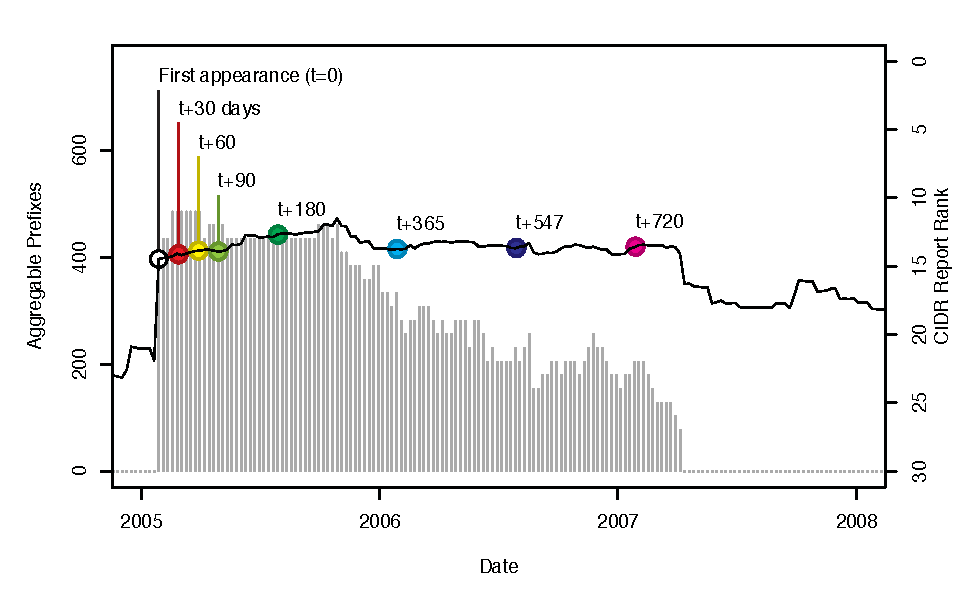
\includegraphics[width=6in]{figures/single_as.pdf}
    \vspace{-2em}\\
    \caption[Illustration of the sampling approach used to measure AS
    behavior]{Illustration of the sampling approach used to measure AS
    behavior, showing the first appearance (shown by the vertical bars
    indicating ranking on the authoritative CIDR Report) and samples at various
    durations thereafter. In this case, aggregable prefixes (netgain) are
    sampled from AS 3602.}
    \label{fig:sample_ex}
\end{centering}
\end{figure}

With these samples collected, differences are then calculated for each of these
quantities relative to the first appearance to understand the behavior change
of the AS relative to its initial appearance. Visualizations and analyses of
these differences and other composite measures created using them are presented
in the next chapter.

\subsection{Establishing the control group}

The process above, explained in terms of the treatment group of ASes that
appear on the authoritative CIDR Report, is identical for the control group,
with the exception of identification of ``appearances'' for the control group,
as the ASes that compose the control group never appear on the CIDR Report.
Instead, appearances in the control group must be constructed. In attempt to
avoid biased construction of the control group, the control group is
constructed randomly as follows.

First, a candidate set of ASes that are elligible to form the control group is
established based on the following elligibility criteria:

\begin{itemize}
    \item{An AS must announce at least 10 prefixes into the routing table in
    order to be elligible. This is an arbitrary minimum threshold, but it is
    intended to exclude the large proportion of stub ASes in the routing table
    that announce single prefixes \cite{6447-table-report}. The implications of
    the selection of this threshold is discussed further in the validity
    section of the next chapter.}
    \item{An AS must be continuously visible in the routing table for a minimum
    of 2 years (720 days) to enable full sampling of its behavior.}
\end{itemize}

From the set of candidate ASes matching this criteria, a number of ASes equal
to the number of ASes appearing on the authoritiative CIDR Report are randomly
selected to form the control group. Finally, for each AS within the control
group, the date of first ``appearance'' is randomly selected between the AS'
first appearance in the routing table and 720 days before it's last appearance
in the routing table. With these appearances established, the sampling and
difference calcluation for the control group proceeds as with the treatment
group.
